\section{Koordinaten Transformation}
\begin{minipage}{0.5\linewidth}
    \subsection{Transformation}
    \begin{minipage}{0.39\linewidth}
        \textbf{Gelenkkoord.}\newline
        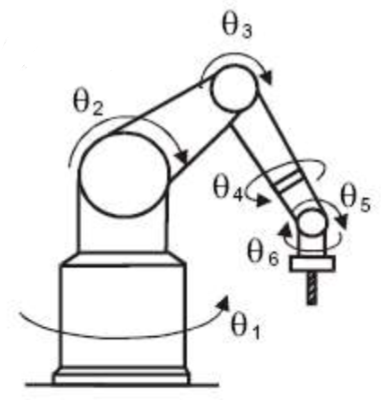
\includegraphics[height=3cm]{./bilder/koordtrans1}
    \end{minipage}
    \begin{minipage}{0.19\linewidth}  
          
        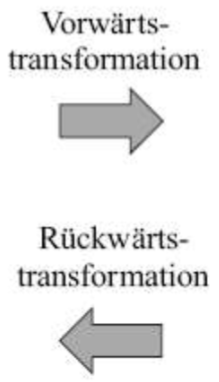
\includegraphics[height=3cm]{bilder/koordtrans2}
    \end{minipage}
    \begin{minipage}{0.39\linewidth}
        \textbf{Globale kart. Koord.}\newline
        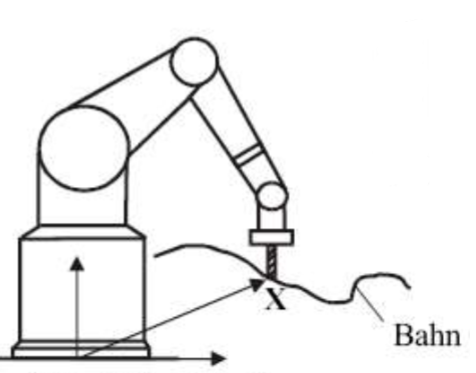
\includegraphics[height=3cm]{./bilder/koordtrans3}
    \end{minipage}
\end{minipage}
\begin{minipage}{0.5\linewidth}
\subsection{Koordinatensysteme}
\begin{tabular}{|c|c|}
    \hline
    Auf Greifer (TCP) & Auf Werkstück\\
    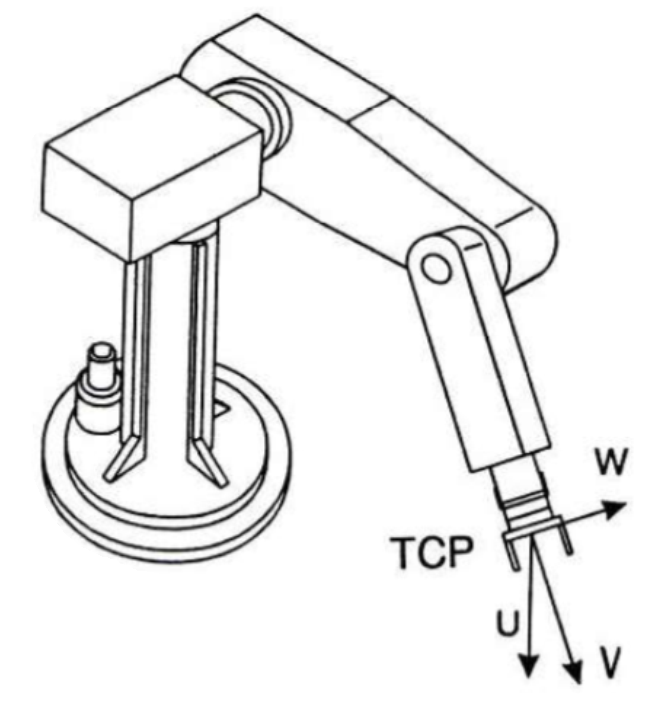
\includegraphics[height=3cm]{./bilder/koordsys1a} & 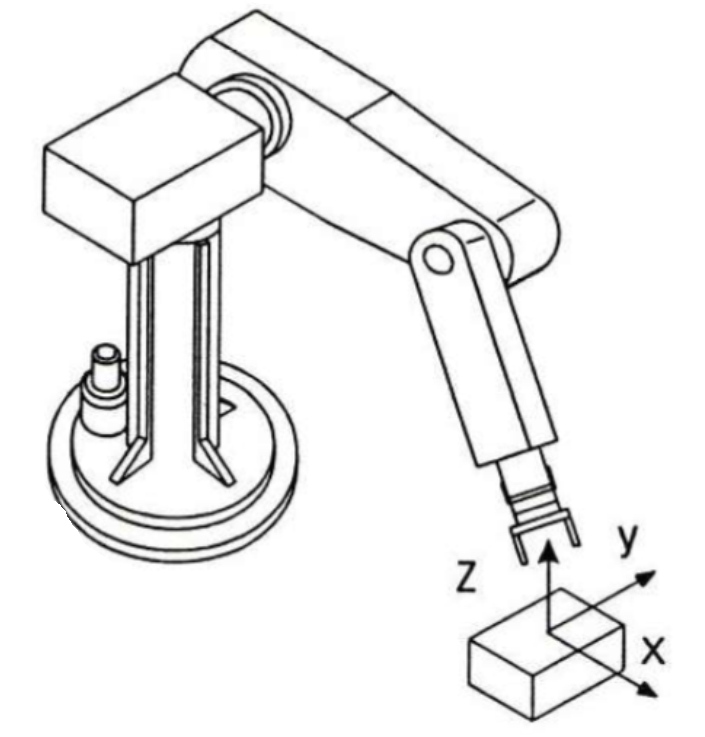
\includegraphics[height=3cm]{./bilder/koordsys1b}\\
    \hline
    Auf Drehaschse 1-6 & Auf Fusspunkt (Raumfest)\\
        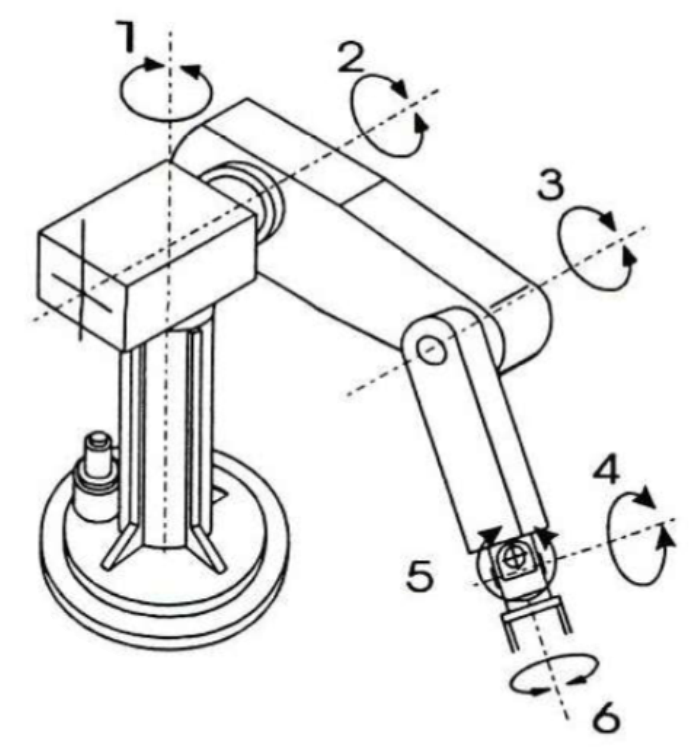
\includegraphics[height=3cm]{./bilder/koordsys1c} & 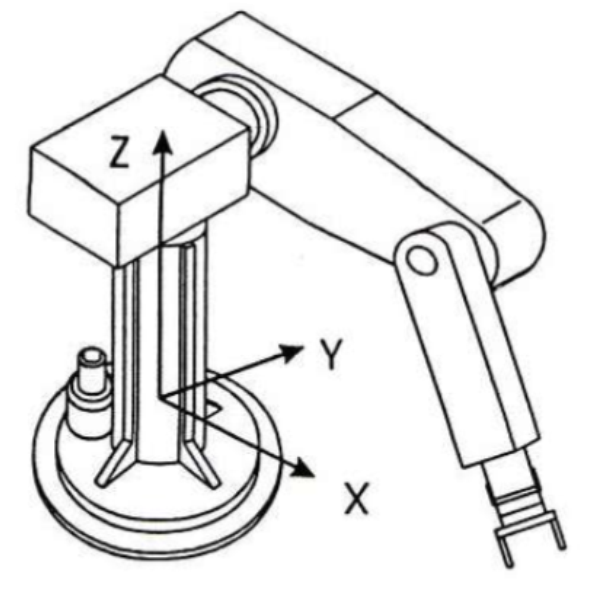
\includegraphics[height=3cm]{./bilder/koordsys1d}\\
    \hline
\end{tabular}
\end{minipage}
\begin{multicols}{2}
    \begin{minipage}{\linewidth}
        \subsubsection{Gelenkkoordinaten}
        \vspace{-1cm}
        \[ q=\begin{bmatrix}
        q_1\\
        q_2\\
        \vdots\\
        q_n
        \end{bmatrix} \]
        \begin{tabular}{ll}
            $q_i = \theta_i$ & Winkel für Drehgelenke\\
            $q_i = d_i$& Verschiebung für Schubgelenke\\
        \end{tabular}
    \end{minipage}

    \begin{minipage}{\linewidth}
        \subsubsection{Kartesische Koordinaten}
        \vspace{-1cm}
        \[ X= \begin{bmatrix}
            {}^0 P_{T_x}\\
            {}^0 P_{T_y}\\
            {}^0 P_{T_z}\\
            \alpha\\
            \beta\\
            \gamma
            \end{bmatrix}           
    \begin{array}{@{\kern-\nulldelimiterspace}l@{}}
          \left.\begin{array}{@{}c@{}}
              \vphantom{\vdots}\\
              \vphantom{\vdots}\\
              \vphantom{\vdots}
          \end{array}\right\}
          \parbox{20em}{Position des Ursprungs von \{T\} in \{O\}\\
          $\rightarrow$Beschreibt die Lage des TCP }\\
          \left.\begin{array}{@{}c@{}}
              \vphantom{\vdots}\\
              \vphantom{\vdots}\\
              \vphantom{\vdots}
          \end{array}\right\}\parbox{20em}{z.B. Euler Winkel\\
              $\rightarrow$Beschreibt die Orientierung des Greifers }\\
      \end{array}
        \]
    \end{minipage}
\end{multicols}

\clearpage
\subsection{Denavit-Hartenberg}
\begin{minipage}{19cm}
    \textbf{Ablauf:}
    \begin{enumerate}{\setlength{\itemsep}{0cm}\setlength{\parsep}{0cm} \setlength{\topsep}{0cm}}
        \item Gelenke nummerieren in aufsteigender Reihenfolge, inkl. Effektor. Starten in der Basis mit Nummer null.
        \item Jeden Achskörper mit Koordinatensystem belegen.
        \item Die $z_i$-Koordinatenachse muss mit der i+1 Gelenkachse zusammenfallen.
        \item Die $x_i$-Achse liegt entlang der Normalen zwischen der $z_{i-1}$ und $z_i$-Achse und zeigt vom Gelenk i zum Gelenk i+1.
        \item $y_i$-Achsen vervollständigen mit der Rechten-Hand-Regel. (x:Daumen, y:Zeigfinger, z:Mittelfinger)
        \item Festlegen der DH-Parameter (siehe DH-Parameter) und eintragen in DH-Tabelle.
        \item DH-Matrizen berechnen und miteinander mulitplizieren.
    \end{enumerate}
    \vspace{0.2cm}
\end{minipage}\\

\begin{minipage}{19cm}
    \textbf{Anmerkung Koordinatensysteme:}
    \begin{itemize}\itemsep0pt
        \item $z_i$-Achse muss grundsätzlich mit Bewegungsachse des zugehörigen Achskörper zusammenfallen.
        Bei Rotationsgelenken gilt die Rechte-Handregel für Drehungen. 
        \item Ursprung des Koordinatensystems im Schnittpunkt der Bewegungsachsen.
    \end{itemize}
    \vspace{0.2cm}
\end{minipage}\\

\begin{minipage}{19cm}
    \textbf{DH-Parameter:}\\ \\
    \begin{tabular}{l l}
        Linklänge $a_i$ (Fixwert): 				& Für $z_{i-1}$ und $z_i$ Achse wird die gem. Normale mit Länge $a_i$ in $x_i$-Richtung gemessen.\\
        Linkdrehung $\alpha_{i}$ (Fixwert):		& Drehwinkel um $x_i$-Achse bis $z_{i-1}$- und $z_i$-Achse in gleiche Richtung zeigen.\\
        Link Offset $d_i$ (Variable):			& Abstand von $x_{i-1}$- und $x_i$-Achse entlang der $z_{i-1}$-Achse.\\
        Gelenkwinkel $\theta_{i}$ (Variable):	& Drehwinkel um $z_{i-1}$-Achse bis $x_{i-1}$- und $x_i$-Achse in gleiche Richtung zeigen.\\
    \end{tabular}
    \vspace{0.5cm}
\end{minipage}\\
\begin{minipage}{19cm}
    \textbf{DH-Tabelle:}\\ \\
    \begin{minipage}{10cm}
        \renewcommand{\arraystretch}{1.1}
        \begin{tabular}{| c | c | c | c | c |}
            \hline
            \textbf{Gelenk Nr.}
            & \textbf{Linklänge $a_i$}
            & \textbf{Linkdrehung $\alpha_{i}$}
            & \textbf{Link Offset $d_i$} 
            & \textbf{Gelenkwinkel $\theta_{i}$}\\
            \hline
            i =1
            &&&& \\
            \hline
            i+1
            &&&& \\
            \hline
            \ldots
            &&&&\\
            \hline
        \end{tabular}
        \renewcommand{\arraystretch}{1}
        \vspace{0.5cm}
    \end{minipage}
\end{minipage}\\
\begin{minipage}{19cm}
    \textbf{DH-Matrizen:}\\ \\
    $ ^{i-1}_{i}T =
    \begin{bmatrix}
    cos(\theta_i) & -sin(\theta_i) cos(\alpha_i) &  sin(\theta_i) sin(\alpha_i) & a_i cos(\theta_i)\\
    sin(\theta_i) &  cos(\theta_i) cos(\alpha_i) & -cos(\theta_i) sin(\alpha_i) & a_i sin(\theta_i)\\
    0			  &  sin(\alpha_i)				 &  cos(\alpha_i)				& d_i\\
    0			  &  0							 &  0							& 1\\
    \end{bmatrix}
    \qquad
    ^{0}_{n}T = \prod\limits_{i=1}^{n} \quad ^{i-1}_{i}T(\theta_{i}) = ^{0}_{1}T \cdot ^{1}_{2}T \cdot \ldots \cdot ^{n-1}_{n}T $
\end{minipage}\\

\begin{minipage}{3cm}
    \textbf{Beispiel:}
    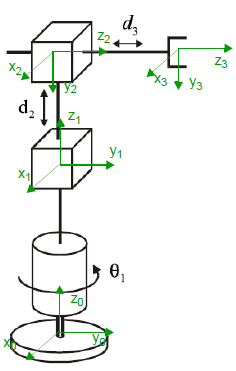
\includegraphics[width=4cm]{./bilder/denavit_grafik.png} \\
\end{minipage}
\begin{minipage}{6cm}
    $\alpha_{i} \Longrightarrow $ Linkdrehung  \\
    $ a_{i} \Longrightarrow $ Linklänge [Achsenabstand] \\
    $ d_{i} \Longrightarrow $ Offset \\
    $ \Theta_{i} \Longrightarrow $ Gelenkwinkel \\ 
\end{minipage}
\begin{minipage}{8cm}
    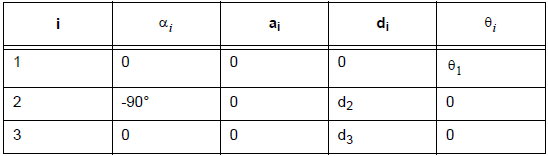
\includegraphics[width=9cm]{./bilder/denavit_tabelle.png} \\
    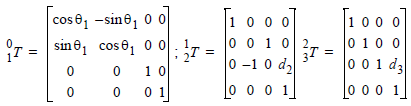
\includegraphics[width=9cm]{./bilder/denavit_matrix.png} \\
\end{minipage} \\